%! Author = snaens
%! Date = 3/2/23

\documentclass[a4paper, 12pt, final]{article} %TODO: draft → final

\usepackage{amsmath}
\usepackage[a4paper,
    left=3cm,
    top=3cm,
    bottom=25mm,
    right=2cm]{geometry}
\usepackage{biblatex}
\usepackage{graphicx}
\usepackage{wrapfig}
\usepackage[german]{babel}
\usepackage{csquotes}
\usepackage{caption}
\usepackage[hang,flushmargin]{footmisc}
\usepackage[hidelinks]{hyperref}
\usepackage{pdfpages}
\usepackage{attachfile}

\graphicspath{ {../media/} }
\addbibresource{FdPB.bib}

% Schriftzug einrichten
\usepackage{tgadventor}
\renewcommand*\familydefault{\sfdefault}
\usepackage[T1]{fontenc}
\usepackage{color}


\title{Der Flug der Pusteblume}
\author{Samuel Pelz}
\date{2023}

\captionsetup[figure]{font=small,labelfont=small}
\begin{document}

    %! suppress = EnDash
    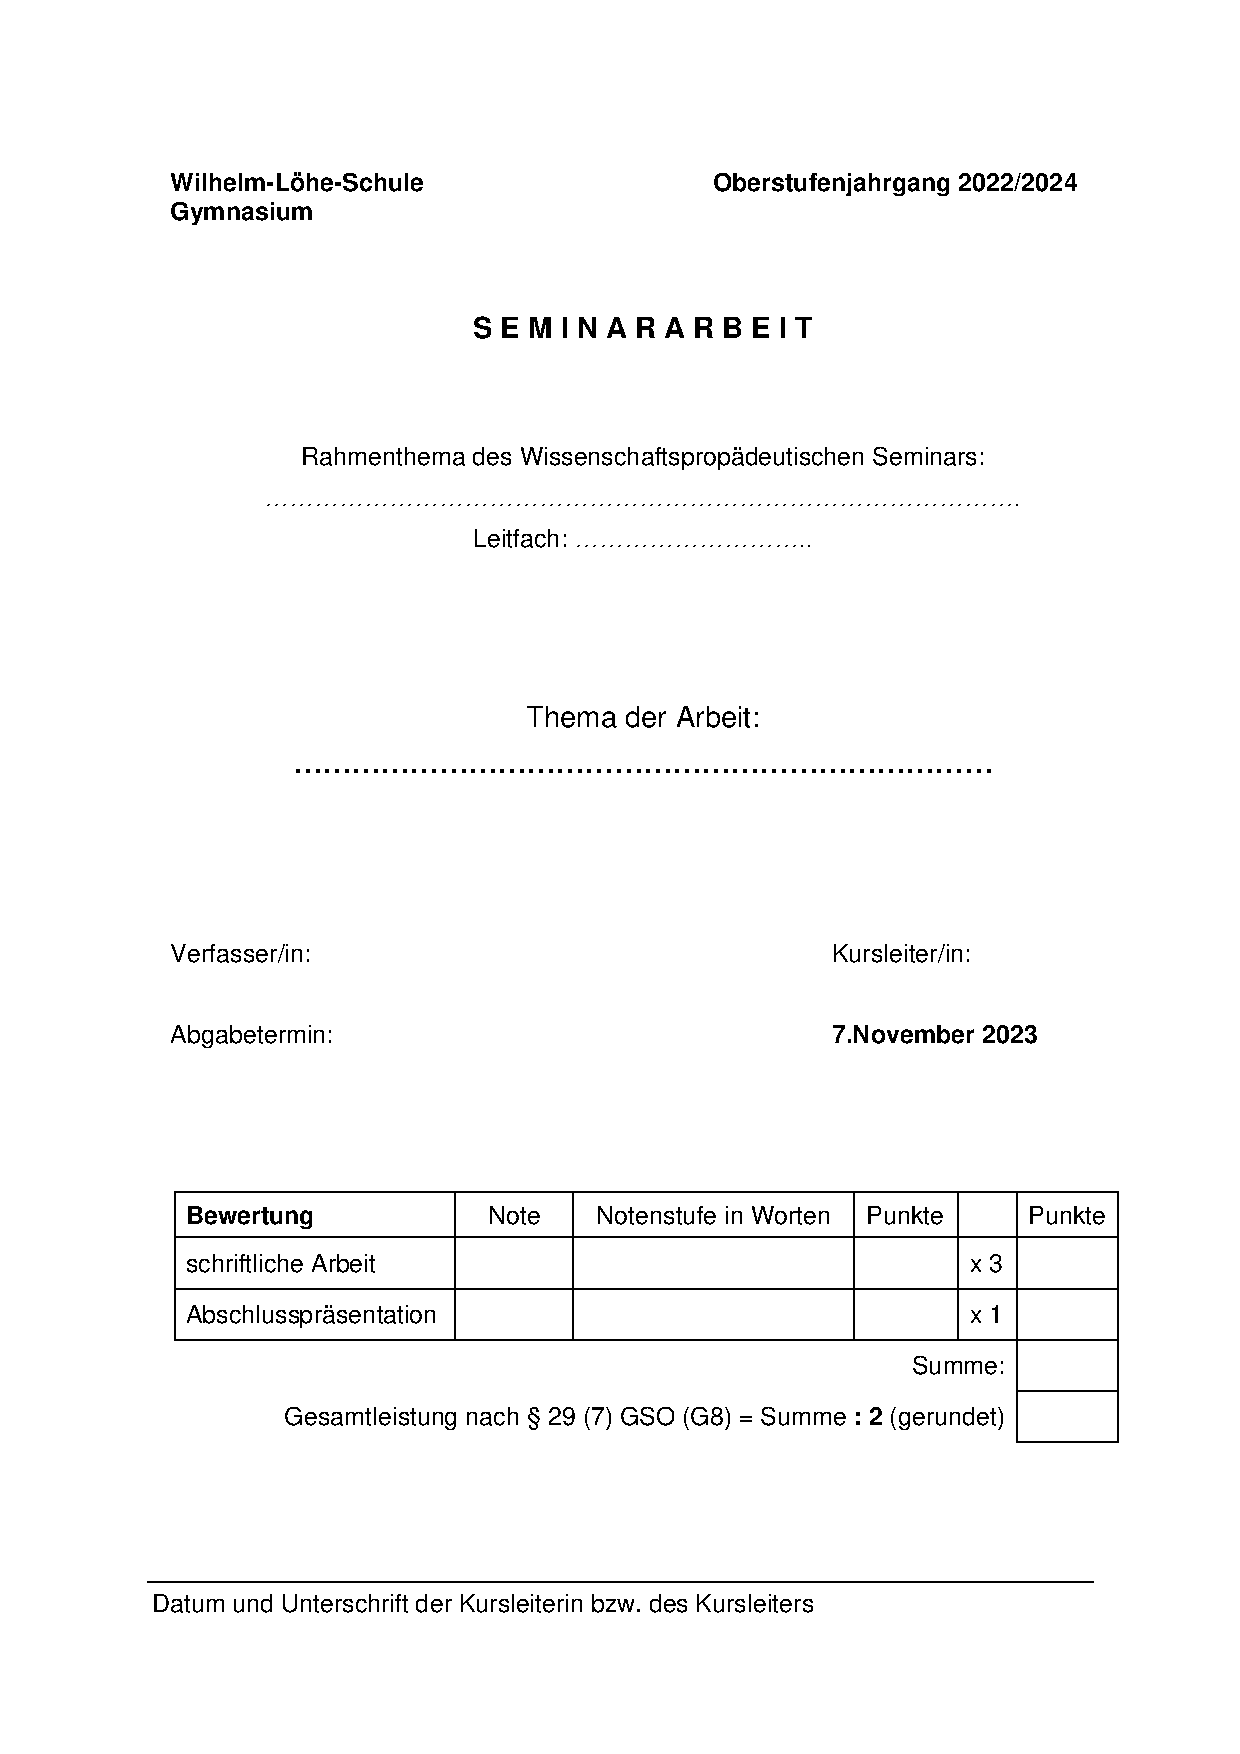
\includepdf{Deckblatt_Seminararbeit 22-24.pdf}
    \newpage


    \maketitle%%%%%%%%%%%%%%%%%%%%%%%%%%%%%%%%%%%%%%%%%%%%%%%%%%%%%%%%%%%%%%%%%%%%%%%%%%%%%%%%%%%%%%%%%%%%%%%%%%%%%%%%%%
    \vspace{3cm}
    \begin{center}
        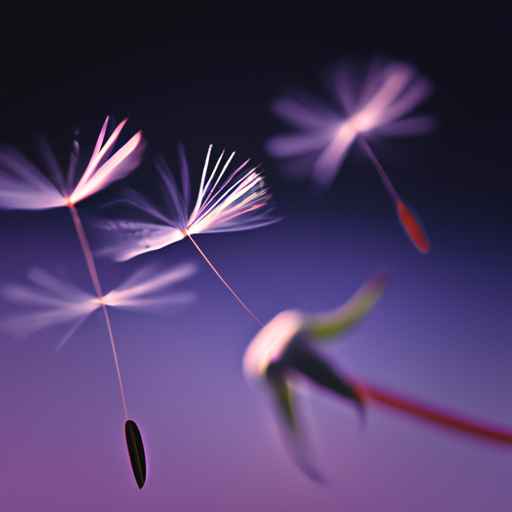
\includegraphics[width=0.75\textwidth]{pusteblume_5}
    \end{center}
    \newpage


    \tableofcontents%%%%%%%%%%%%%%%%%%%%%%%%%%%%%%%%%%%%%%%%%%%%%%%%%%%%%%%%%%%%%%%%%%%%%%%%%%%%%%%%%%%%%%%%%%%%%%%%%%%%
    \listoffigures
    \newpage


    \section{Einleitung}\label{sec:einleitung}%%%%%%%%%%%%%%%%%%%%%%%%%%%%%%%%%%%%%%%%%%%%%%%%%%%%%%%%%%%%%%%%%%%%%%%%%%

    \enquote{Ich beobachtete fasziniert den Flug [der Pusteblume] und war beeindruckt von der Leichtigkeit des Fliegens.}\footfullcite{ach_pusteblume}\\
    Es ist erstaunlich, wie leicht die Pusteblume fliegt.
    Ein leichter Windstoß reicht aus, um überall ihre Samenflieger zu verteilen,
    die dann mit dem Wind weite Distanzen zurücklegen können.
    Diese sonderbaren Fähigkeiten der Pflanze haben sofort Neugier in mir geweckt.
    Wie schafft sie das, und auch vollkommen passiv, ohne bewegung?\\
    Die Pusteblume symbolisiert wohl nicht umsonst loslassen und Leichtigkeit\footfullcite{ach_pusteblume}, oder?
    \newpage


    \section{Die Pusteblume}\label{sec:untersuchung-der-pusteblume}%%%%%%%%%%%%%%%%%%%%%%%%%%%%%%%%%%%%%%%%%%%%%%%%%%%%%
    Pusteblume ist der Kosename für den Löwenzahn, auch \textit{Taraxacum (officinale)} genannt.
Hierbei handelt es sich um Pflanzen der Familie der Korbblütler,
die \enquote{weltweit von den Tropen bis zu den Polargebieten verbreitet}\footfullcite{Taraxacum} auffindbar sind.\\

\noindent
Ihren globalen Erfolg haben sie vor allem ihrer Fortpflanzung zu bedanken,
denn sie sind fähig sich asexuell zu vermehren, und können pro Pflanze bis zu 20.000 Diasporen, die jeweils kilometerweit fliegen können, erzeugen.\footfullcite{wisc-dandelion}\footcite{Taraxacum}


\begin{figure}[h]
    \centering
    \begin{minipage}{0.45\textwidth}
        \centering
        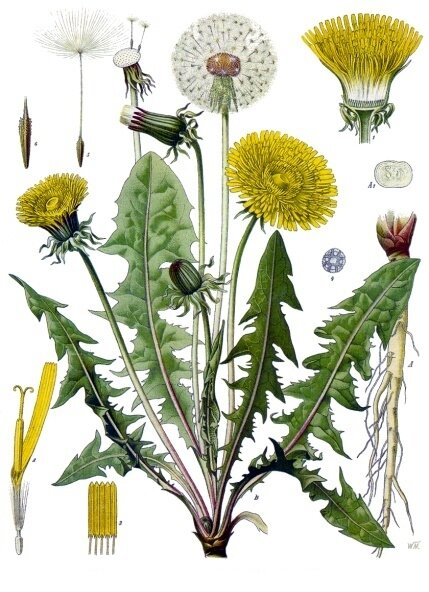
\includegraphics[width=\textwidth]{Drawing-representing-the-life-cycle-of-Taraxacum-officinale-2}
        \caption{Taraxacum officinale\cite[, Fig 2.1]{tesi}}
    \end{minipage}
    \hfill
    \begin{minipage}{0.5\textwidth}
        \centering
        \setbox0\hbox
        {\includegraphics[width=\textwidth]{achäne-schema}}
        \ht0=10cm % change this to move it up or down
        \dp0=0cm
        \box0
        \caption{Eine Achäne \cite[\textit{in Anlehnung an}][, Fig 1.1]{tesi}}
        \label{fig:figure3}
    \end{minipage}
\end{figure}

\newpage

\subsection{Achäne}\label{subsec:achane}

Wie in Abbildung ~\ref{fig:figure3} veranschaulicht besteht die Achäne - die Diaspore des \textit{Taraxacum officinale} hauptsächlich aus Pappus und Samen.
Die Härchen des Pappus haben mikroskopische Dornen die radial aus den Härchen hervortreten,
und bestehen, ähnlich wie Holz, aus hohlen Röhrchen.\footfullcite{morph}
Diese Konstruktion verleiht den Härchen stabilität und ein geringes Gewicht.

\begin{figure}[h]
    \centering
    \begin{minipage}{0.4\textwidth}
        \centering
        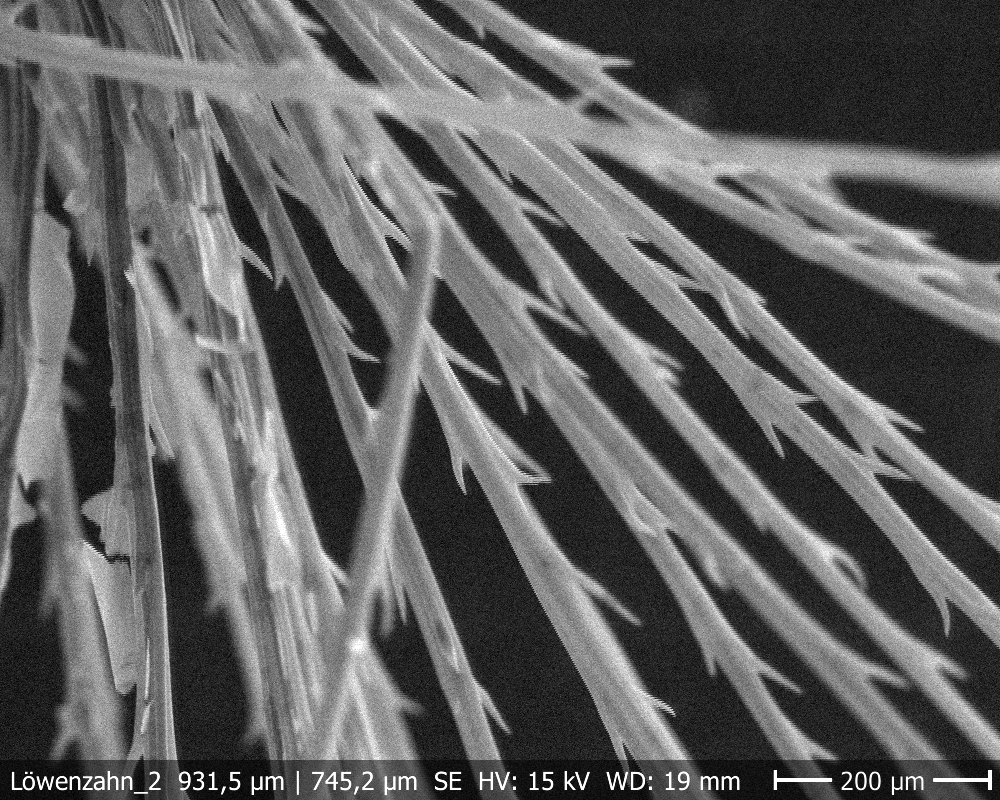
\includegraphics[width=\textwidth]{sam_pusteblume_2}
        \caption{Elektronenmikroskopie der Pappushärchen, [\textit{Eigene Darstellung}]}
        \label{fig:emk_1}
        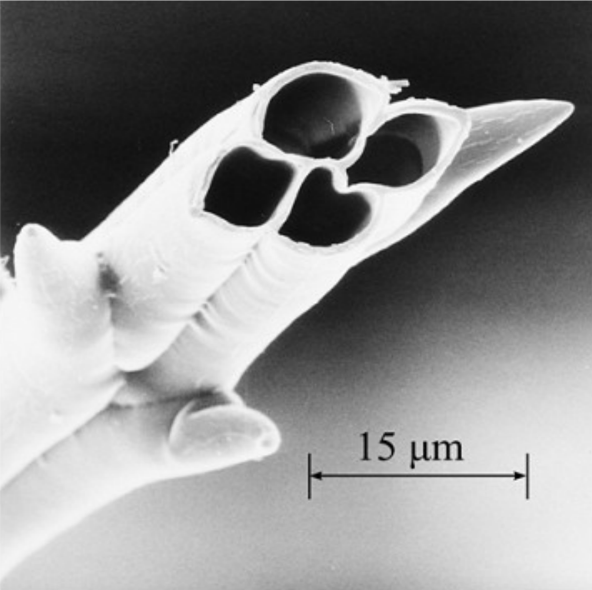
\includegraphics[width=0.8\textwidth]{Pappushaar}%
        \caption{Elektronenmikroskopie der Pappushärchen, \cite[, Fig. 9]{morph}}
        \label{fig:emk_2}
    \end{minipage}
    \hfill
    \begin{minipage}{0.3\textwidth}
        \centering
        \includegraphics[width=\textwidth]{Fallverhalten_achäne}%
        \caption{Fallverhalten der Achäe, \cite[, Fig. 4]{morph}}
        \label{fig:flt}
    \end{minipage}
\end{figure}

Die Positionierung des Samens bewirkt einen tiefen Schwerpunkt vom Flugkörper.
Dadurch richtet er sich im Flug, sodass der Samen unten, und der Pappus oben,
und senkrecht zur Fallrichtung ausrichtet ist, wie in Abbildung ~\ref{fig:flt}.\\
\enquote{Der Pappus [...] fungiert als Fallschirm und ist die Ursache der relativ langsamen Fallgeschwindigkeit.}\footfullcite[(Übersetzt)]{morph}

\newpage


    \section{Aerodynamik}\label{sec:aerodynamik}%%%%%%%%%%%%%%%%%%%%%%%%%%%%%%%%%%%%%%%%%%%%%%%%%%%%%%%%%%%%%%%%%%%%%%%%
    Um das Flugverhalten der Achäne zu untersuchen wurde Schlierenfotografie versucht.

\subsection{Schlieren}\label{subsec:schlieren}

Schlieren entstehen, wenn in einem transparenten Medium eine Homogenitätsstörung hervortritt.\footfullcite{schlieren}
Dies passiert unter anderem bei Bewegungen der Luft, und ist zum Beispiel als `welligkeit' der Luft über heißen Objekten mit dem bloßen Auge sichtbar\footfullcite[0:50]{josh-BOS}.
Im Falle der Löwenzahndiaspore zeigen sie die Luftverwirbelungen an, die beim Flug entstehen.

\subsubsection{BOS}\label{subsubsec:bos}

Background Oriented Schlieren\footnotetext{auf deutsch: Hintergrundorientiertes Schlieren} (BOS) ist ein Verfahren,
mit dem man ohne externe optische Instrumente Schlieren sichtbar machen kann.
\smallskip\\
Hierbei werden zwei Kamerabilder mit statischem Hintergrund verglichen,
wobei das erste Bild als Hintergrund/Referenz benutzt wird, und das zweite die Schlieren erfasst.
Vergleicht man nun die Bilder miteinander zeigt sich, dass im Schlieren-Bild der Hintergrund entlang der verschiedenen Luftströmungen verzerrt ist.
Dies liegt daran, dass Unterschiede in der Dichte der Luft das durchquerende Licht gebrochen haben und erscheint auf einer Kamera als \enquote{Verschiebung der Pixel im Kamerabild}\footfullcite[(Übersetzt), 1:07]{josh-BOS},
welche man mit geeigneter Bildverarbeitung verdeutlichen kann.
\smallskip\\
Für beste Resultate nimmt man das Hintergrundbild vor dem Erscheinen der gesuchten Schlieren.
Sonst werden gleichbleibende Strömungen kaum erfasst, da die Brechung konstant ist.
\bigskip\\
BOS hat den Vorteil, dass nur eine Kamera und ein geeigneter Hintergrund benötigt werden, um Schlierenbilder zu machen.
Dies macht es vom Aufbau her simpler als andere Schlierenfotografieverfahren.
\smallskip\\
Leider trägt dieses Verfahren auch Nachteile mit sich, vor allem, dass der Hintergrund und die Kamera sich nicht bewegen dürfen,
da dies sonst als Störsignal erscheint.
Auch das Kamerabild muss relativ geräuschfrei sein, was eine gute Kamera und Lichtbedingungen voraussetzt.

\begin{figure}[h]
    \centering
    \begin{minipage}{0.5\textwidth}
        \centering
        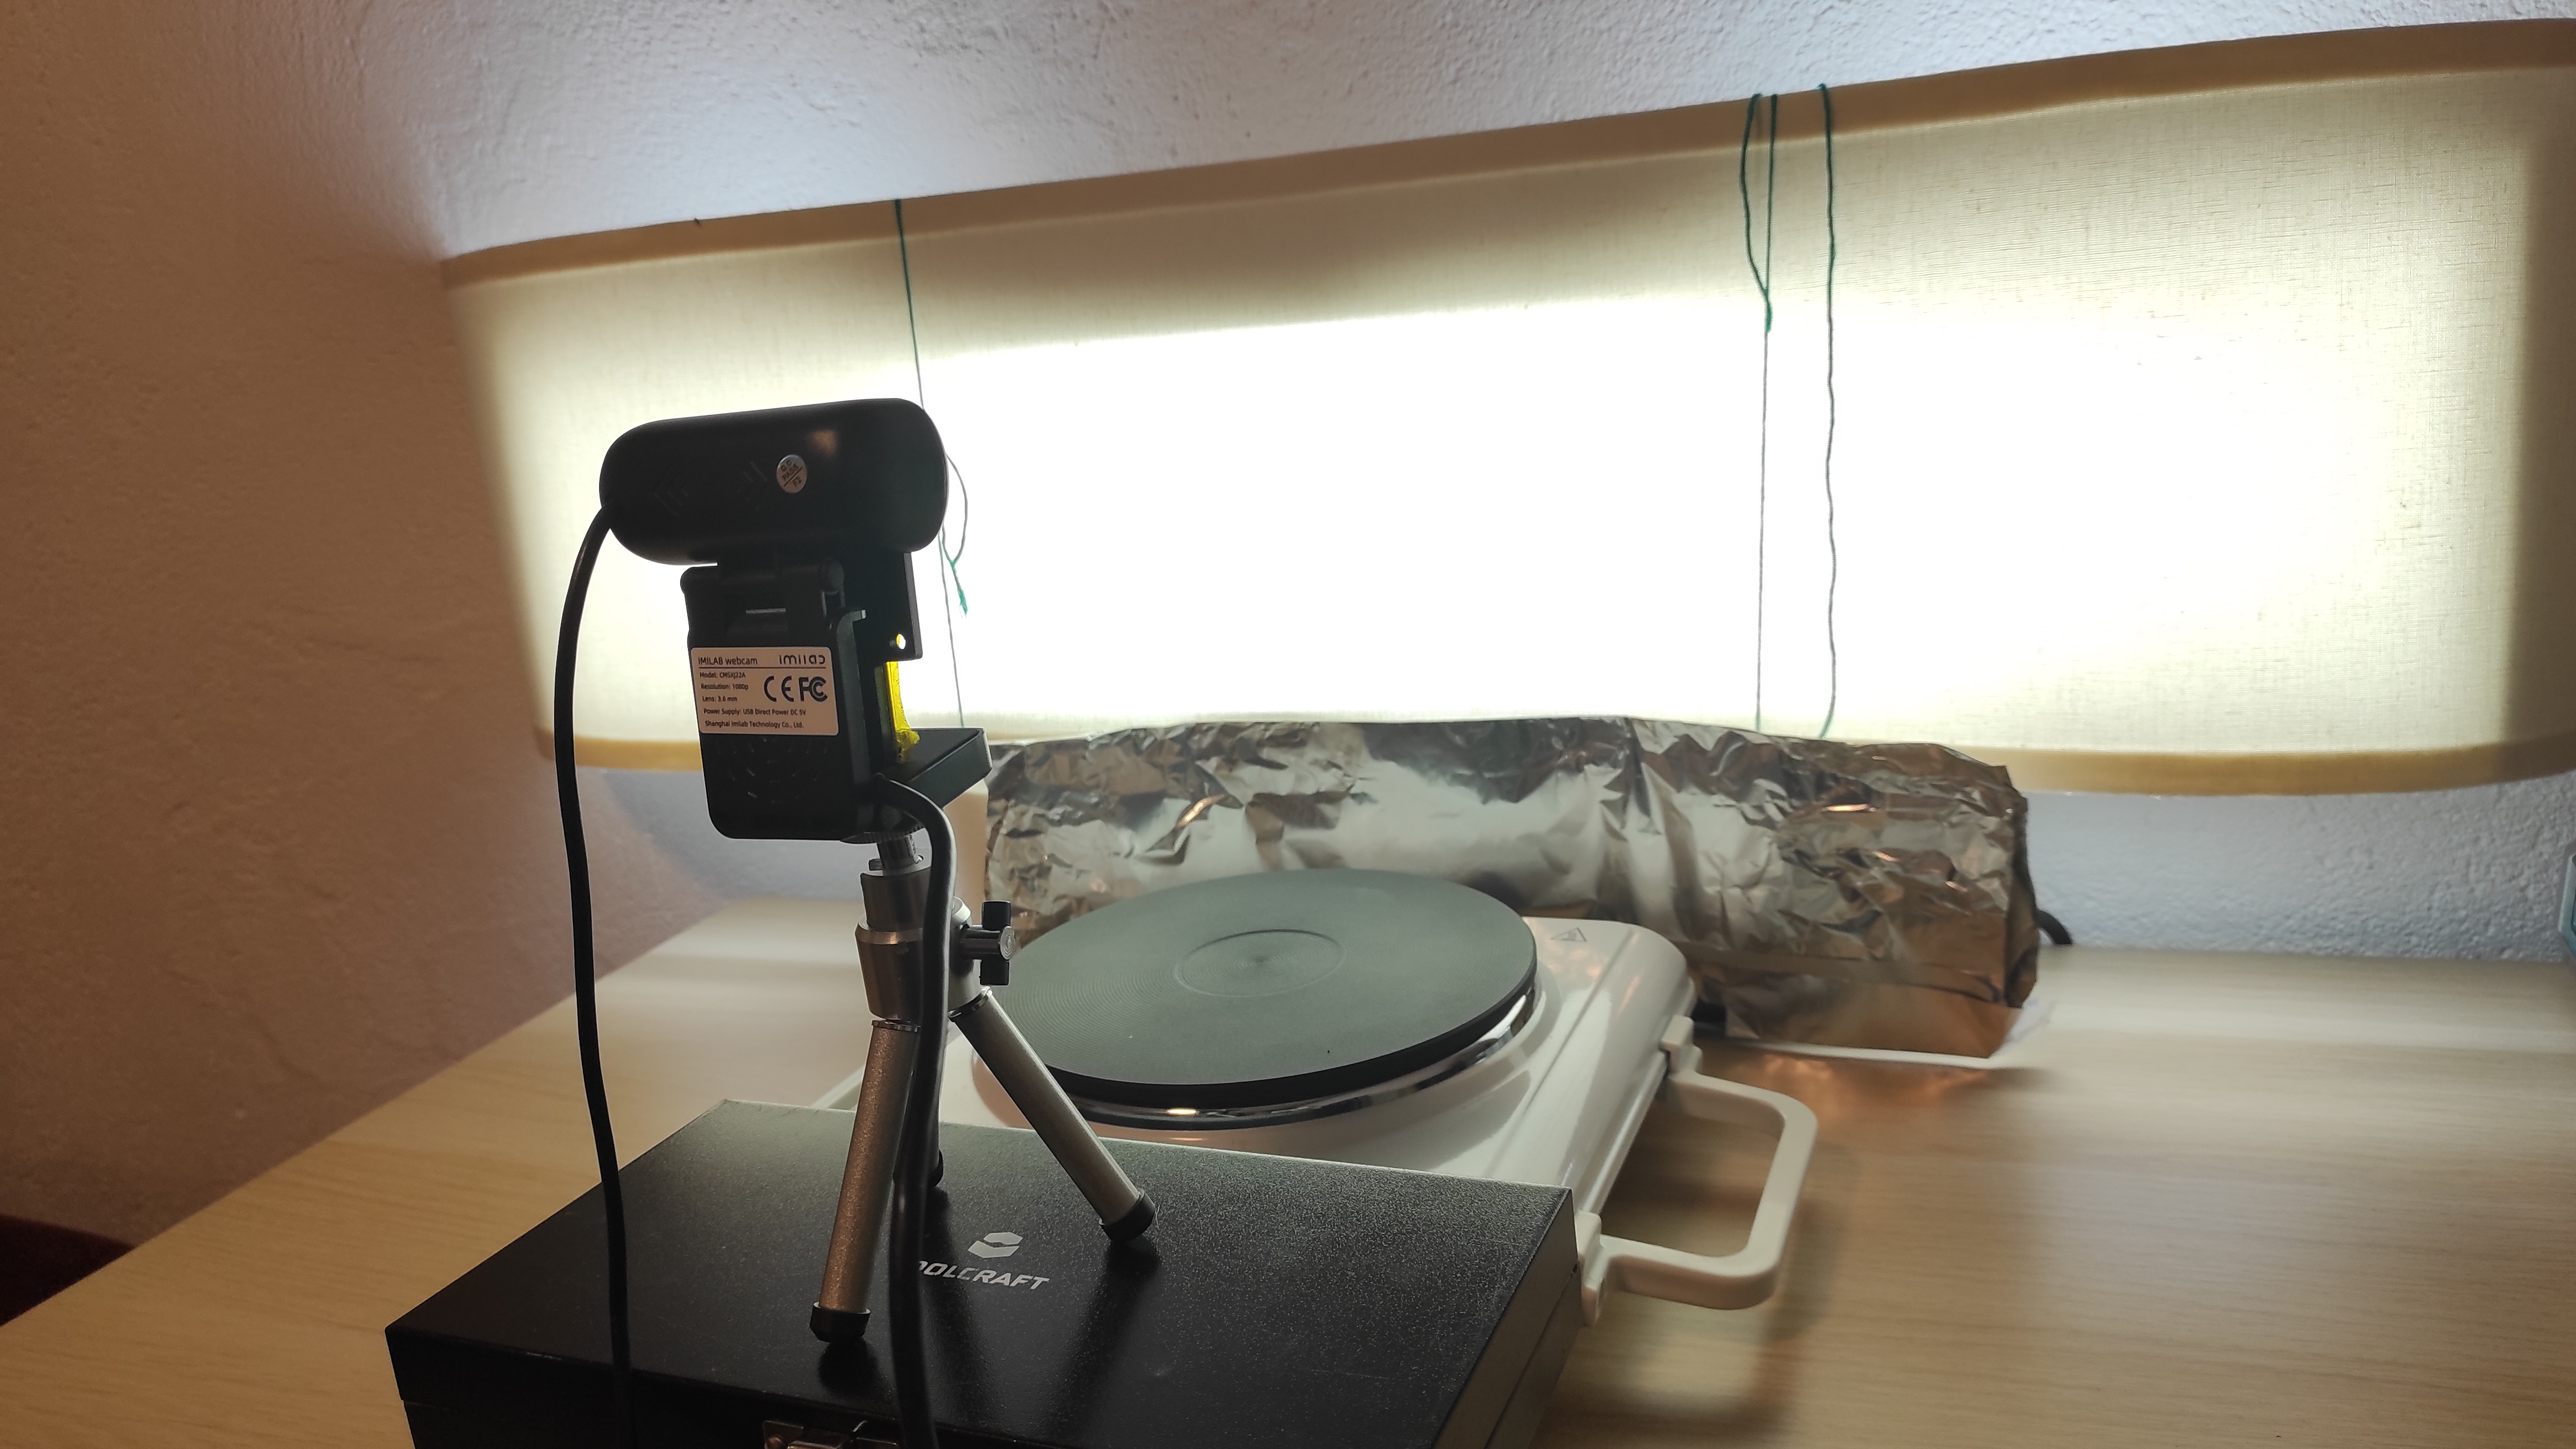
\includegraphics[width=\textwidth]{BOS-setup}
        \caption{Mein BOS setup, [\textit{Eigene Darstellung}]}
        \label{fig:sl_bos1}
    \end{minipage}
    \hfill
    \begin{minipage}{0.4\textwidth}
        \centering
        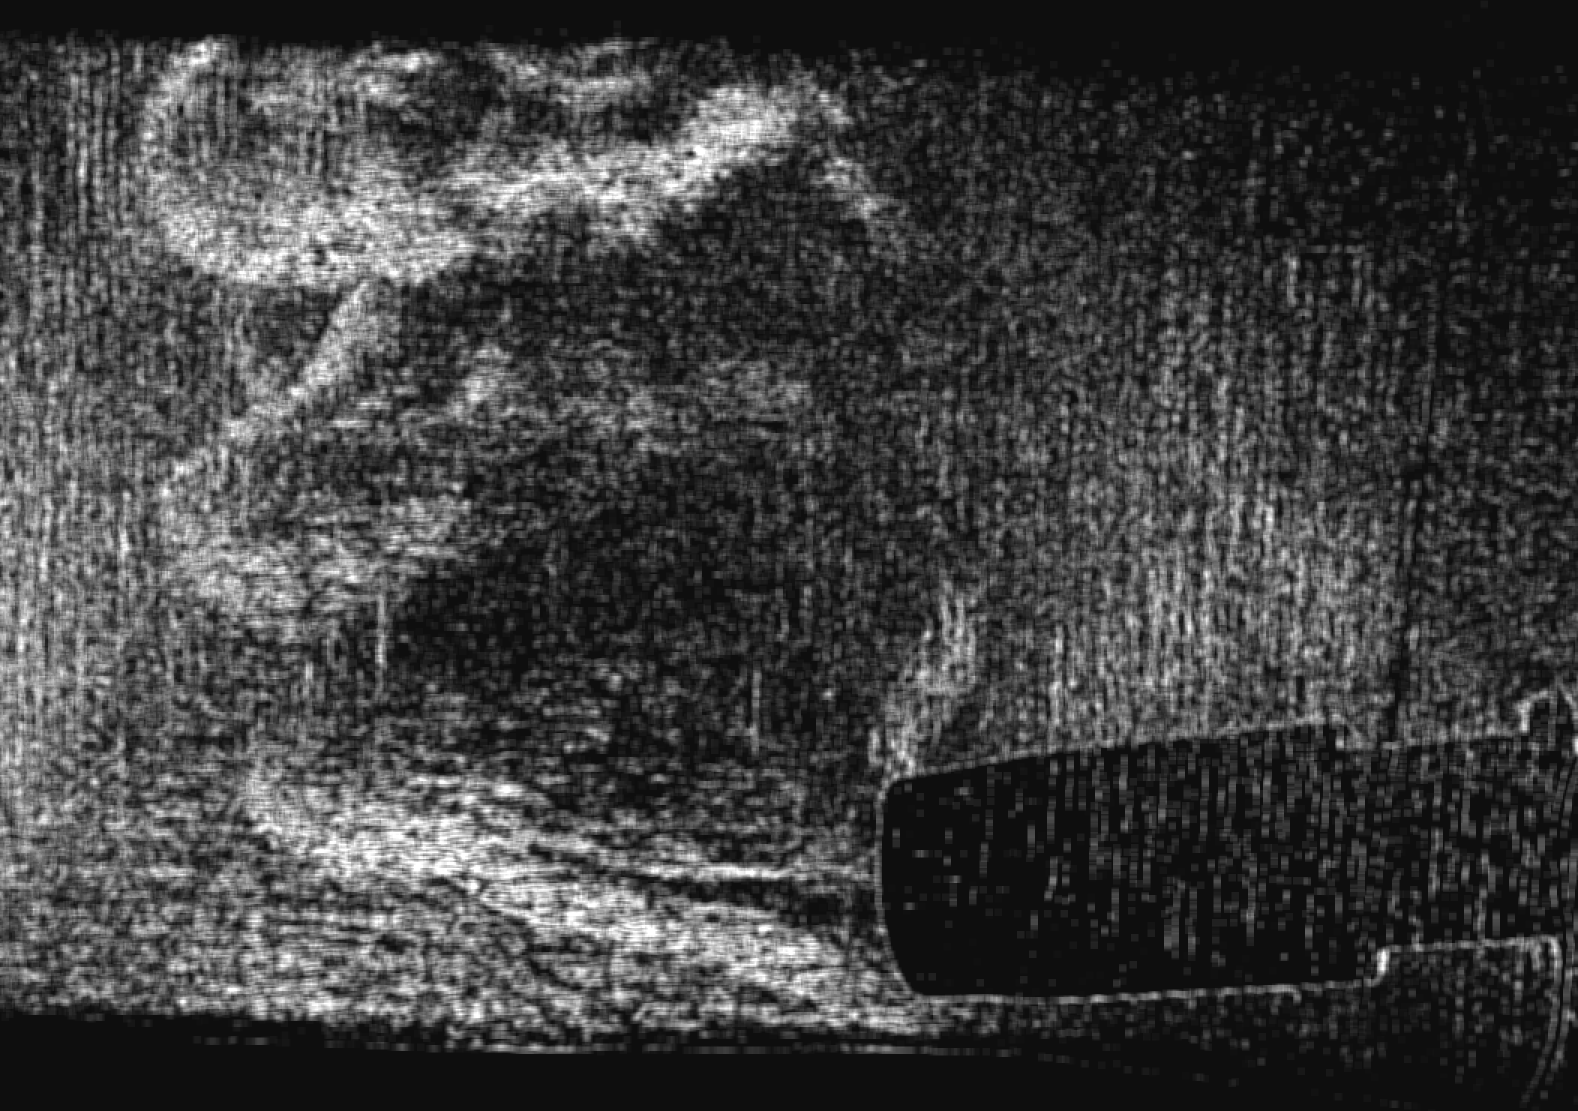
\includegraphics[width=\textwidth]{schliere-flamenwerfer}
        \caption{BOS Bild eines Flammenwerfers, [\textit{Eigene Darstellung}]}
        \label{fig:sl_bos2}
    \end{minipage}
\end{figure}

\newpage

\subsubsection{Ein-Spiegel Schlieren system}\label{subsubsec:ein-spiegel-schlieren-system}

\begin{figure}[h]
    \centering
    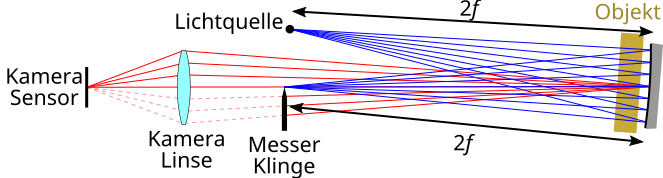
\includegraphics[width=0.8\textwidth]{Single_mirror_schlieren}
    \caption{Ein ein-Spiegel Schlieren system \cite[\textit{in Anlehnung an}][]{esss}}
    \label{fig:esss}
\end{figure}
\noindent
Dieses system benutzt eine Lichtquelle, einen gekrümmten Spiegel und eine Messerklinge um Schlieren zu visualisieren.
\smallskip\\
Die Lichtquelle und Messerklinge werden versetzt, aber trotzdem zum Spiegel gerichtet ausgelegt,
sodass der Brennpunkt des von der Lichtquelle reflektierten Lichts auf die Messerklinge fällt.
Eine geeignete Kamera wird hinter der Messerklinge aufgestellt und deren Fokus auf den Spiegel justiert.
Diese wird die Schlierenbilder nehmen.\\
Nur wenn Licht von Schlieren gebrochen wird kann es die Messerkante überqueren und in die Kamera gelangen.
\smallskip\\
Um das Ausrichten aller Elemente dieser Anordnung zu erleichtern und/oder um den Kontrast der Schlieren einzurichten,
kann man das Messer verstellen um mehr oder weniger des reflektierten Lichtstrahls zu blockieren.
Licht, dass nicht von dem Messer blockiert wurde sorgt für den charakteristischen hellen Hintergrund in einem ein-spiegel Schlieren system.



\newpage
\begin{figure}[h]
    \centering
    \begin{minipage}{0.5\textwidth}
        \centering
        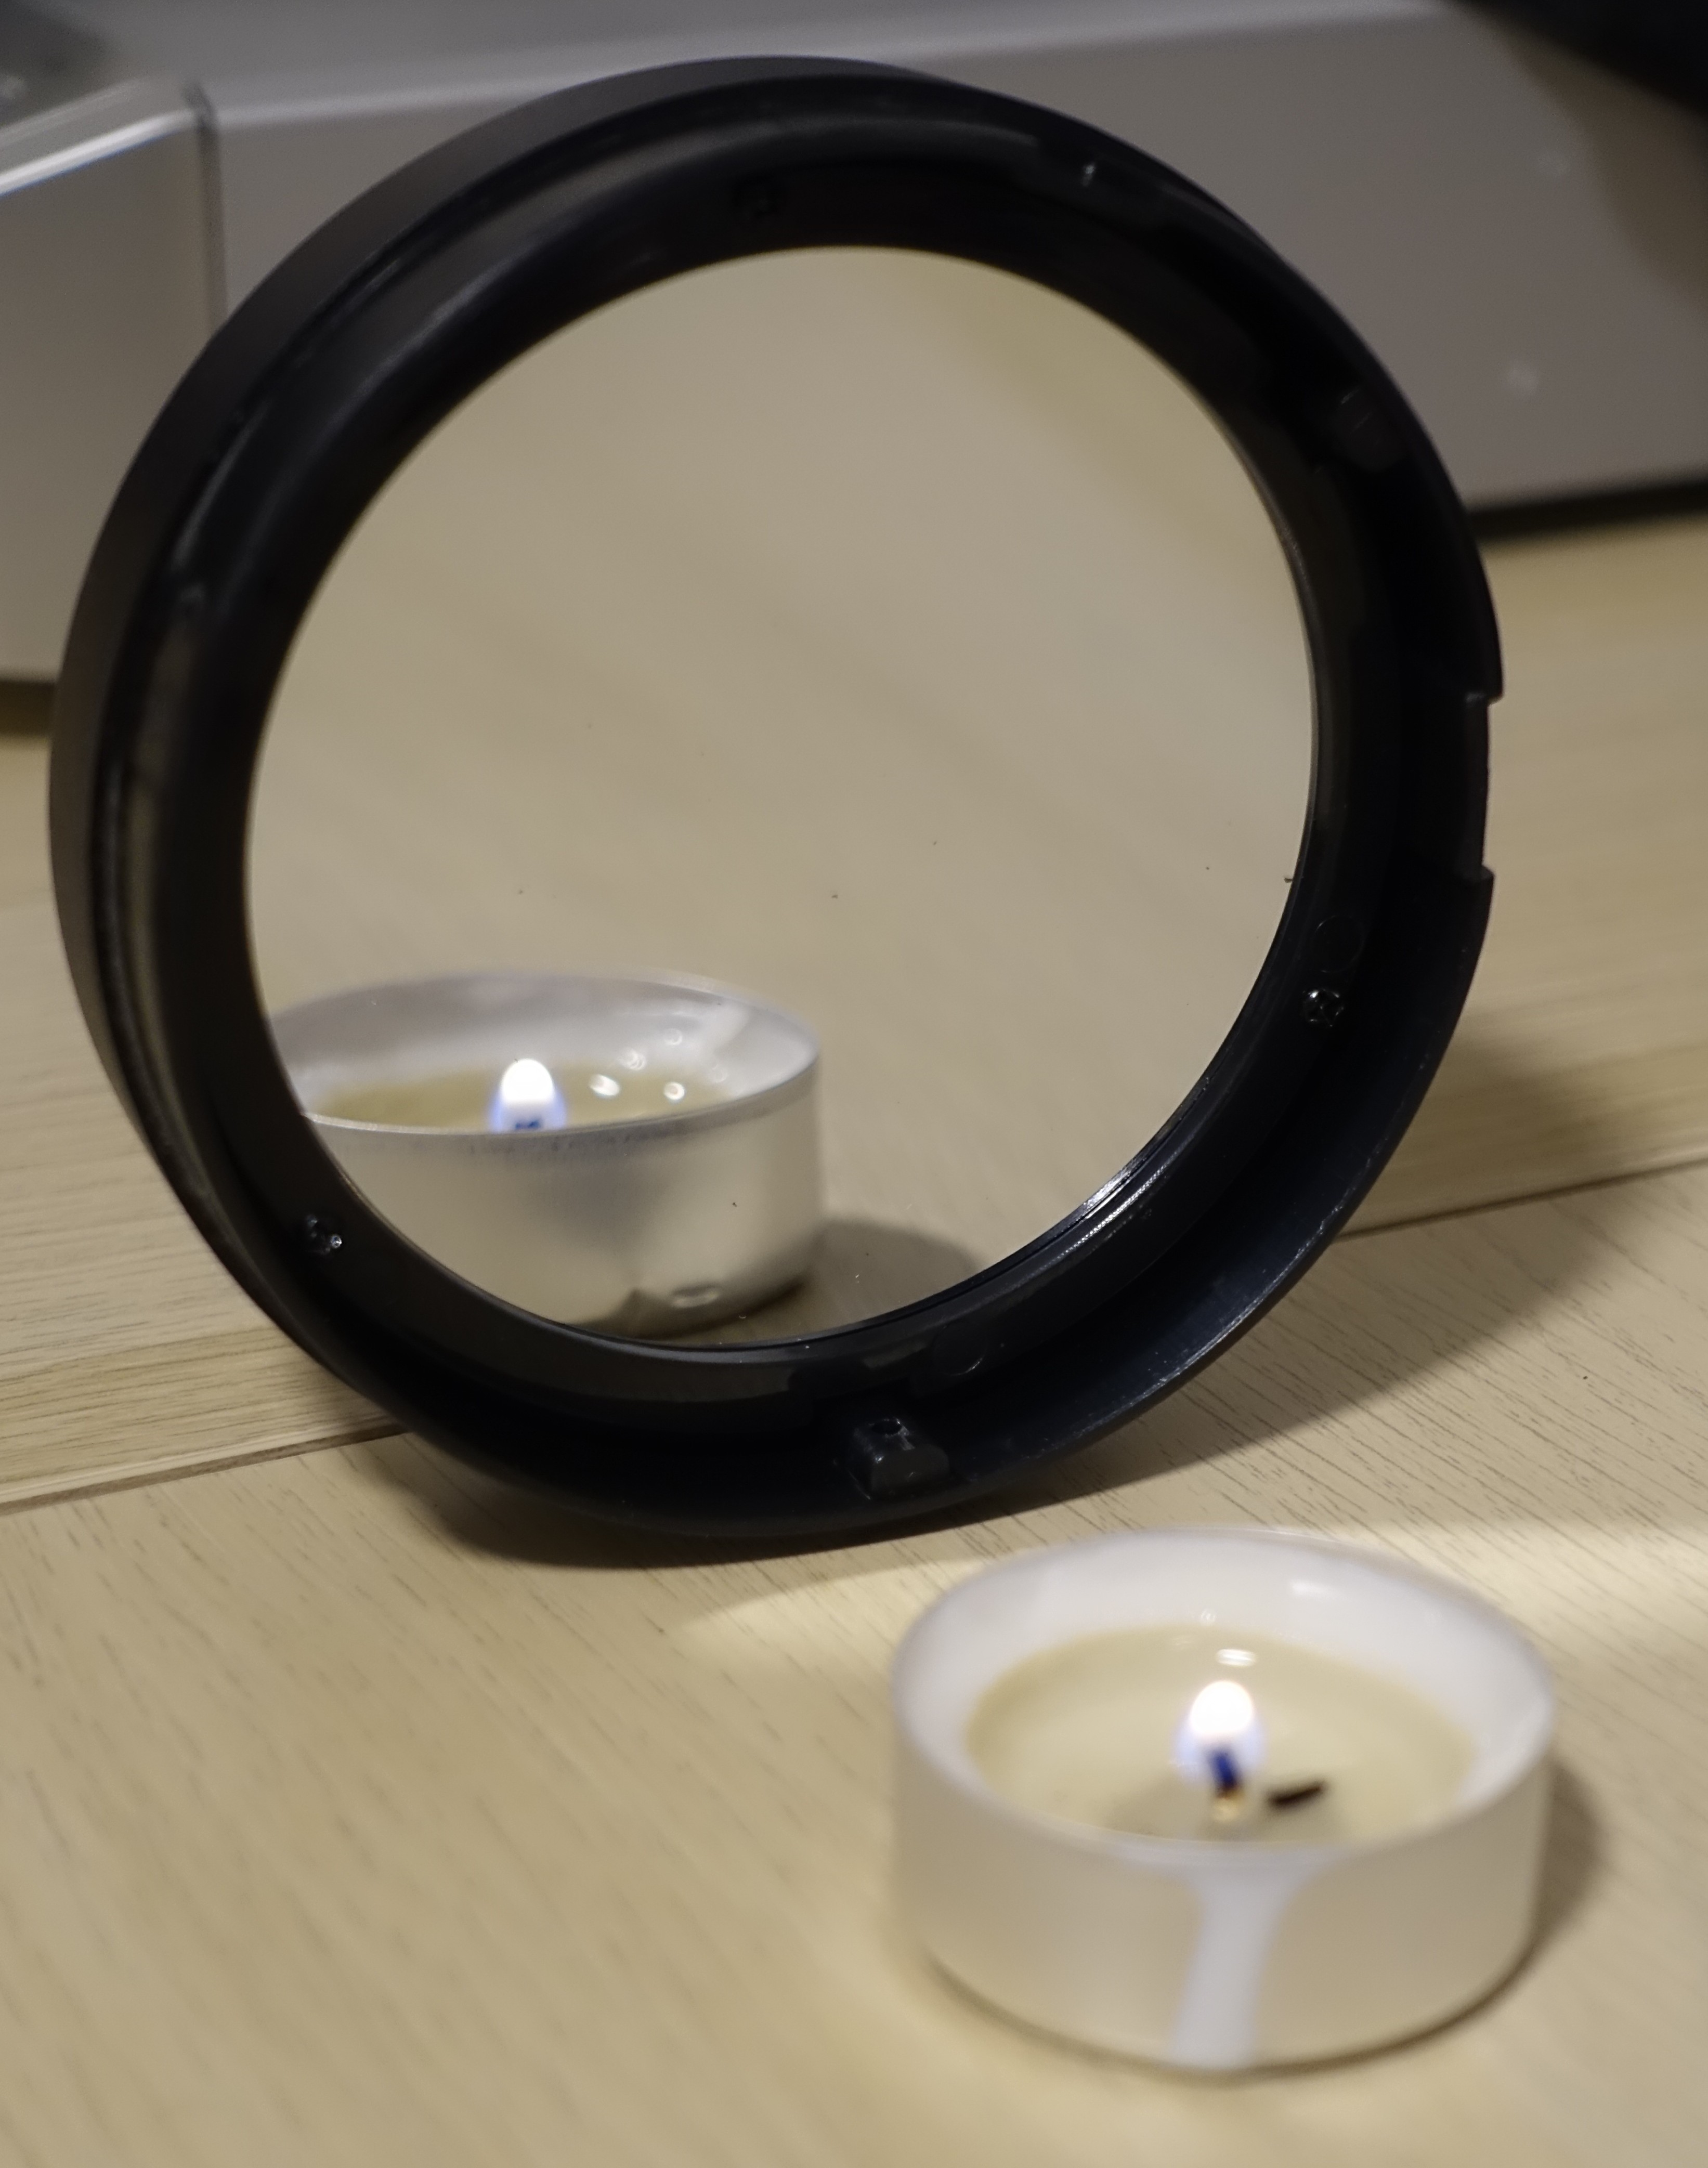
\includegraphics[width=\textwidth]{SL_spiegel_setup}
        \caption{Mein Spiegel, [\textit{Eigene Darstellung}]}
    \end{minipage}
    \hfill
    \begin{minipage}{0.4\textwidth}
        \centering
        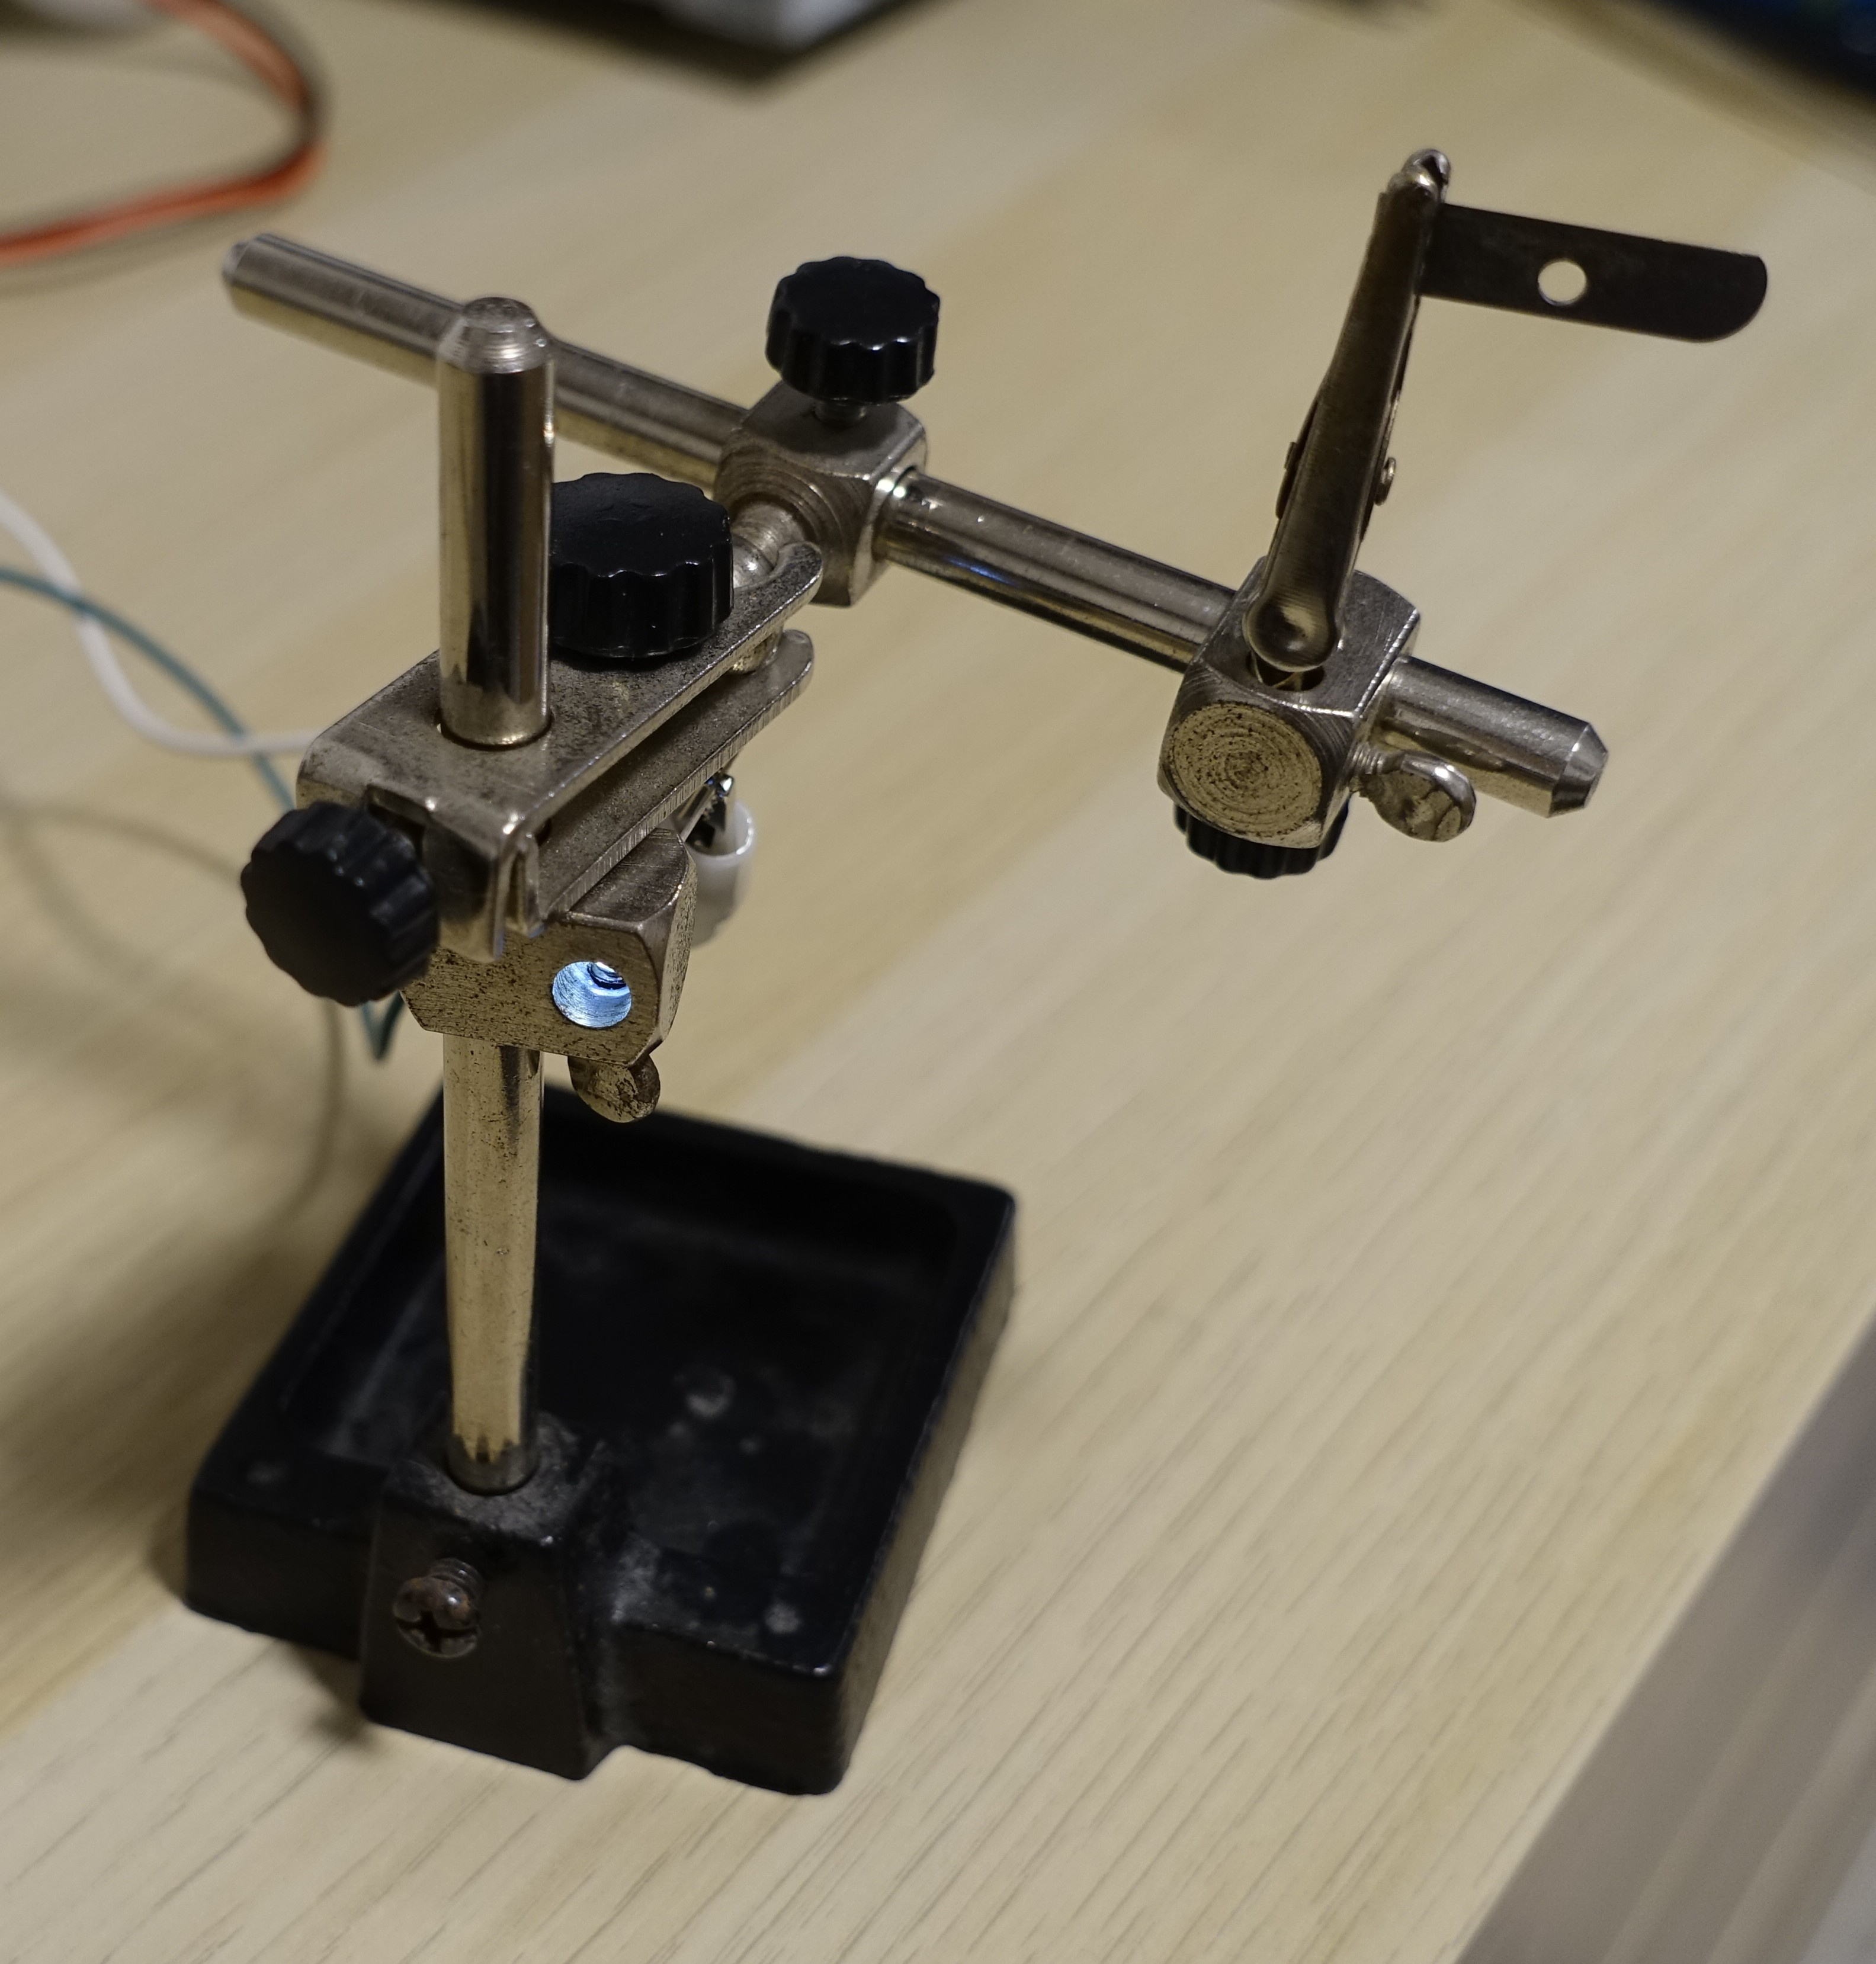
\includegraphics[width=\textwidth]{SL_spiegel_setup_2}
        \caption{Meine Lichtquelle und Messerklinge, [\textit{Eigene Darstellung}]}
    \end{minipage}
    \label{fig:sl_spi}
\end{figure}
\newpage

\subsection{Windtunnel}\label{subsec:windtunnel}

Um die Luftströmungen der Achäne im Flug zu sehen musste eine laminare Windquelle hergestellt werden,
da beide Schlierenverfahren mit fallenden Objekten schwer verwirklichbar wären.\\
Der erste Versuch hierzu war mit einer heizplatte.
Die Hoffnung war einen ähnlichen laminar - turbulent übergang wie die Schlieren der Kerze in Figur ~\ref{fig:sl_heip1} zu bekommen.
Stattdessen konnte nur ein turbulenter Strömungsverlauf gemessen werden, Idee gescheitert.\\

\begin{figure}[h]
    \centering
    \begin{minipage}{0.3\textwidth}
        \centering
        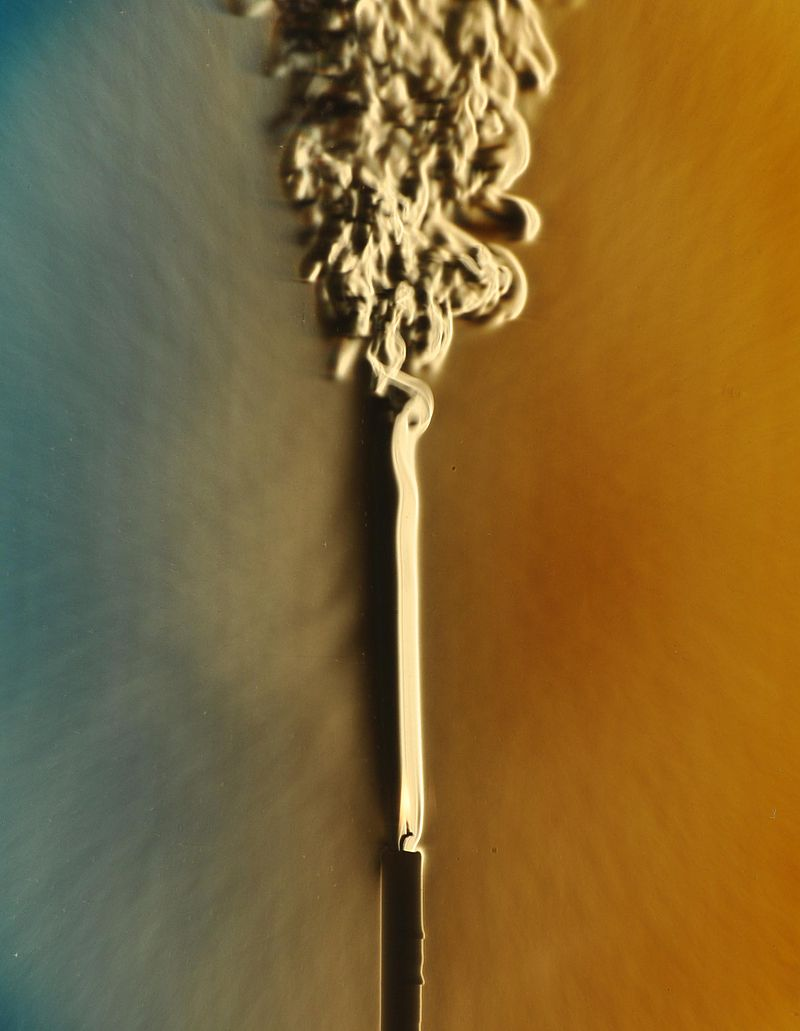
\includegraphics[width=\textwidth]{kerze-schliere}
        \caption{laminar - turbulent übergang an einer Kerze \cite{kerze-schliere}}
        \label{fig:sl_heip1}
    \end{minipage}
    \hfill
    \begin{minipage}{0.6\textwidth}
        \centering
        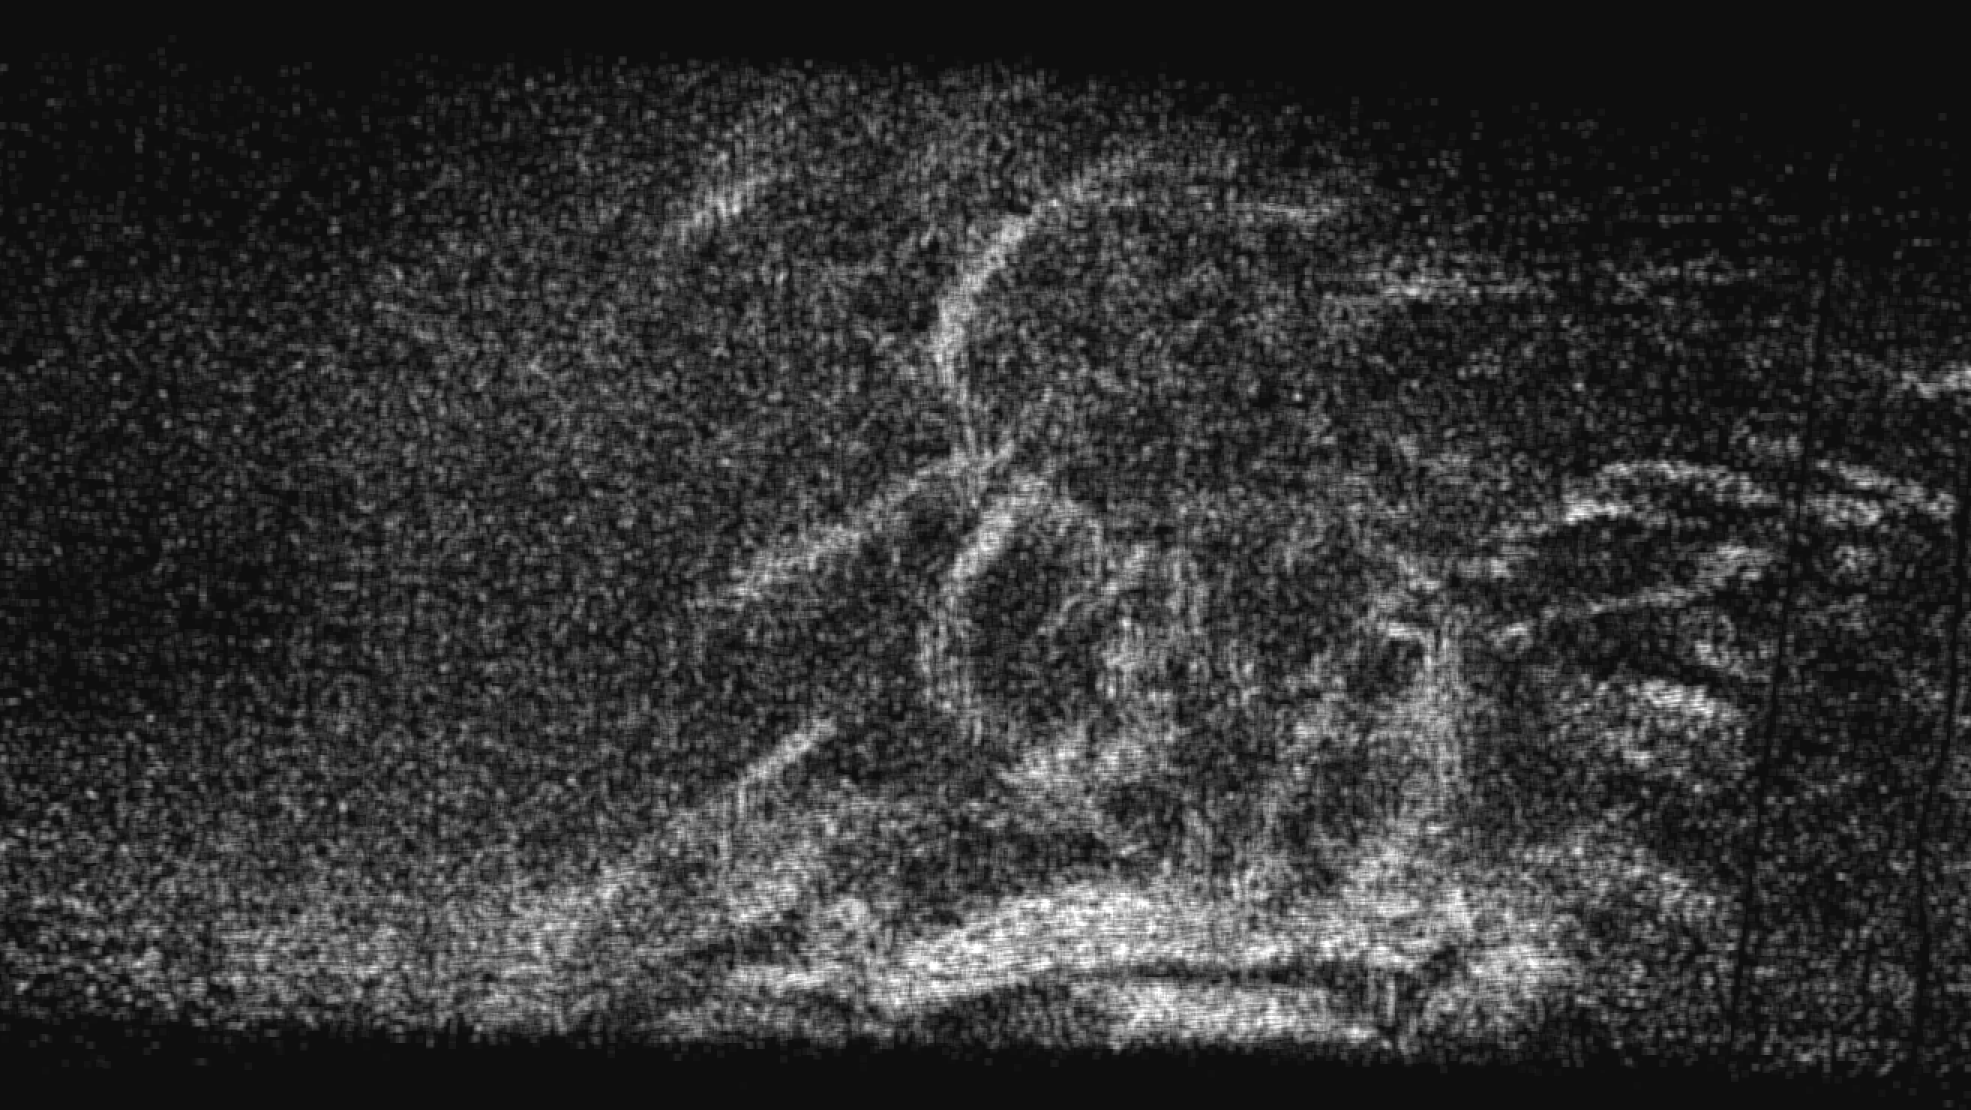
\includegraphics[width=\textwidth]{Heizplatte-BOS}
        \caption{BOS foto von eingeschalteter Heizplatte \ref{fig:sl_bos1}, [\textit{Eigene Darstellung}]}
        \label{fig:sl_heip2}
    \end{minipage}
\end{figure}

\noindent
Nach sehr kurzfristiger Recherche zur besten Art und Weise einen laminaren Luftstrom zu bekommen,
wurde ein Windtunnel geplant, gebaut und getestet.
Hierzu wurde ein 120mm Lüfter als Sogquelle benutzt, und eine Klarsichtfolie als Fenster.

\begin{figure}[h]
    \centering
    \begin{minipage}{0.55\textwidth}
        \centering
        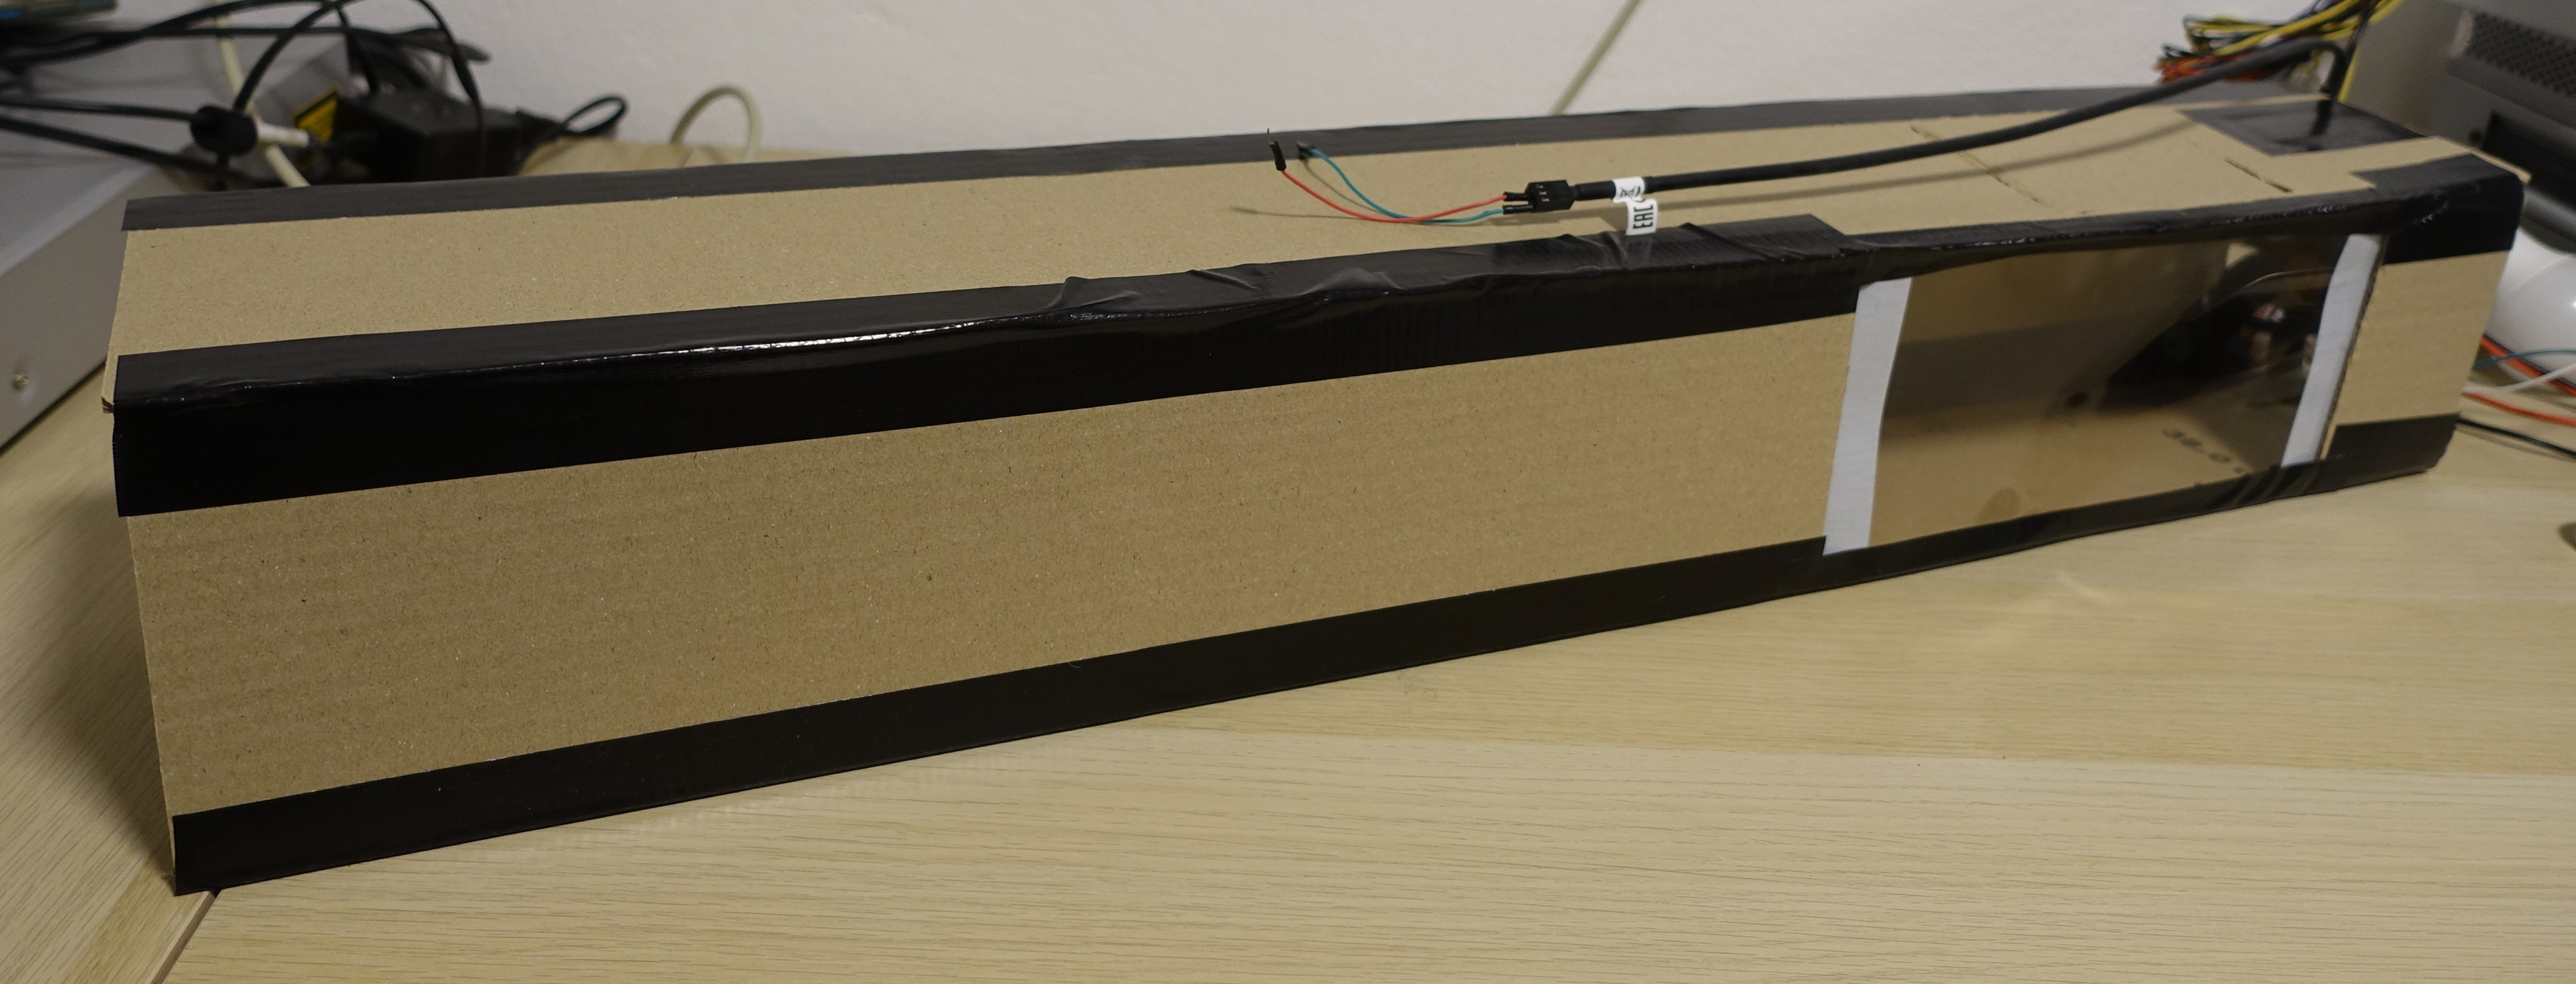
\includegraphics[width=\textwidth]{windtunnel_1}
        \caption{Windtunnel - Außenansicht, [\textit{Eigene Darstellung}]}
        \label{fig:windt1}
    \end{minipage}
    \hfill
    \begin{minipage}{0.4\textwidth}
        \centering
        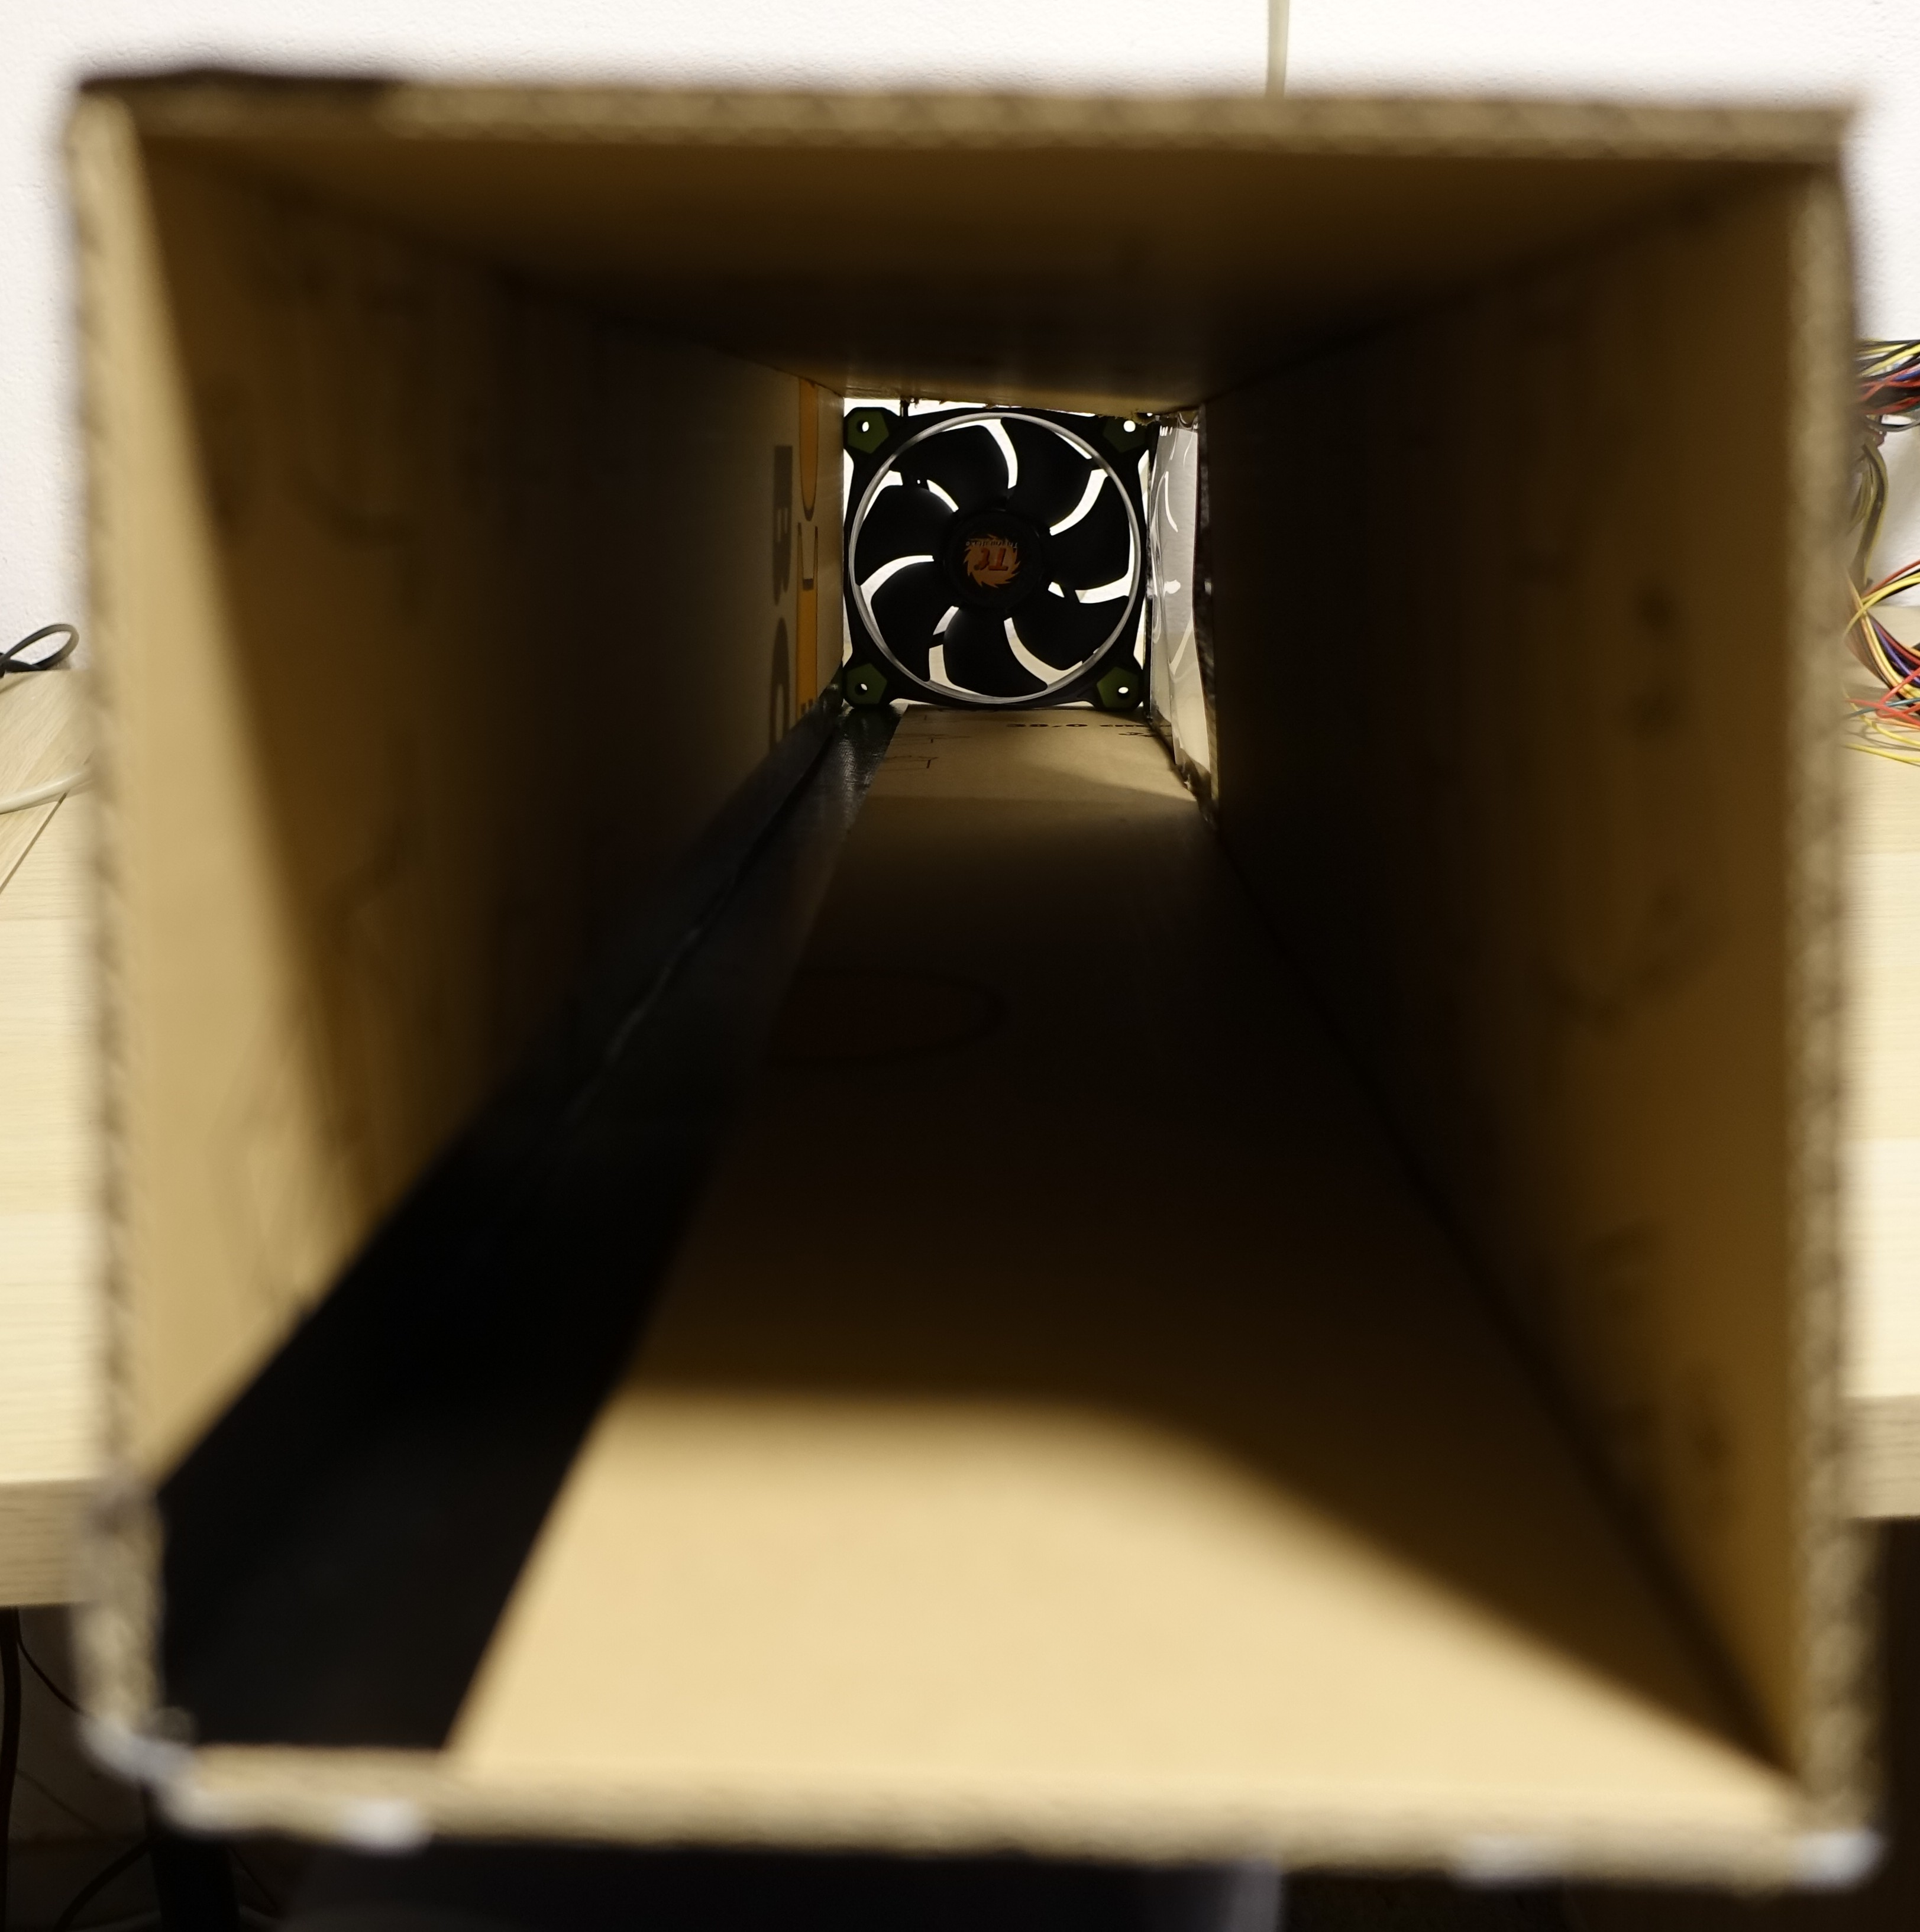
\includegraphics[width=\textwidth]{windtunnel_2}
        \caption{Windtunnel - Innenansicht, [\textit{Eigene Darstellung}]}
        \label{fig:windt2}
    \end{minipage}
\end{figure}

\noindent
Der Windtunnel funktionierte wunderbar, und der Luftstrom der Kerze war fast statisch.

\begin{figure}[h]
    \centering
    \begin{minipage}{0.3\textwidth}
        \centering
        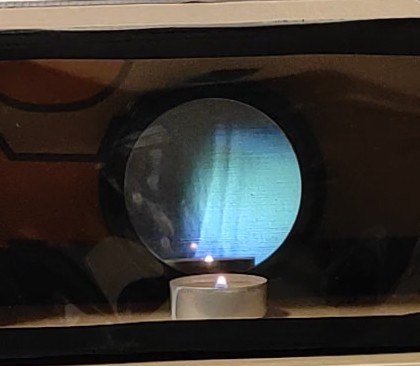
\includegraphics[width=\textwidth]{windt_sl_l}
        \caption{Kerze im Windtunnel - wenig Wind, [\textit{Eigene Darstellung}]}
        \label{fig:windt_sl_l}
    \end{minipage}
    \hfill
    \begin{minipage}{0.3\textwidth}
        \centering
        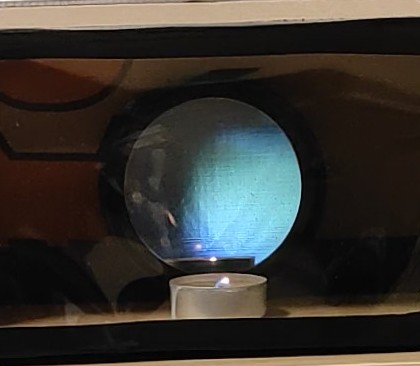
\includegraphics[width=\textwidth]{windt_sl_m}
        \caption{Kerze im Windtunnel - mäßig Wind, [\textit{Eigene Darstellung}]}
        \label{fig:windt_sl_m}
    \end{minipage}
    \hfill
    \begin{minipage}{0.3\textwidth}
        \centering
        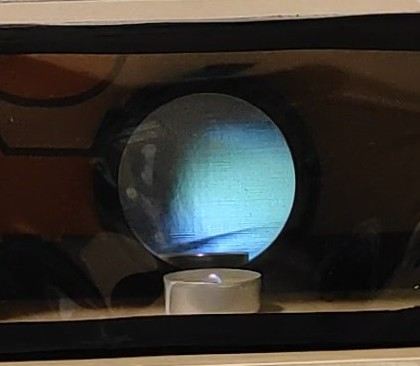
\includegraphics[width=\textwidth]{windt_sl_h}
        \caption{Kerze im Windtunnel - viel Wind, [\textit{Eigene Darstellung}]}
        \label{fig:windt_sl_h}
    \end{minipage}
\end{figure}

\subsection{Resultat}\label{subsec:resultat}

Beide Schlierenfotografiesysteme haben bereits bei Kerzen, welche relativ starke Luftströmungen generieren, die Schlieren nicht zufriedenstellend visualisieren können.
Die wesentlich schwächeren, durch den Pappus ausgelösten verwirbelungen waren mit den genutzten Geräten leider nicht sichtbar.\\
Die am meisten gelungene Aufnahme (Abbildung ~\ref{fig:sl}), wo eine Kerze von unten den Luftstrom generiert,
zeigt nur wie die Luft am Pappus abgelenkt wird, und nicht die erwartete Verwirbelung,
wie sie in Abbildung ~\ref{fig:sl_pro}, ein von profis gemachtes bild, zu sehen ist.

\noindent
Diese Verwirbelung ist, durch die Kreisförmige Obenansicht des Pappus toroidal und bietet so der vorbeiziehenden Luft mehr Widerstand.

\medskip\noindent
Der Algorithmus für die BOS Bilder ist ~\textattachfile{../BOS/BOS.cpp}{\textcolor{black}{\textbf{hier}}} im PDF eingebettet,
oder unter\\ ~\url{https://gist.github.com/snaens/2b34830f7e117739d994411dc2abbc91} erreichbar. \ref


\newpage
\begin{figure}[h]
    \centering
    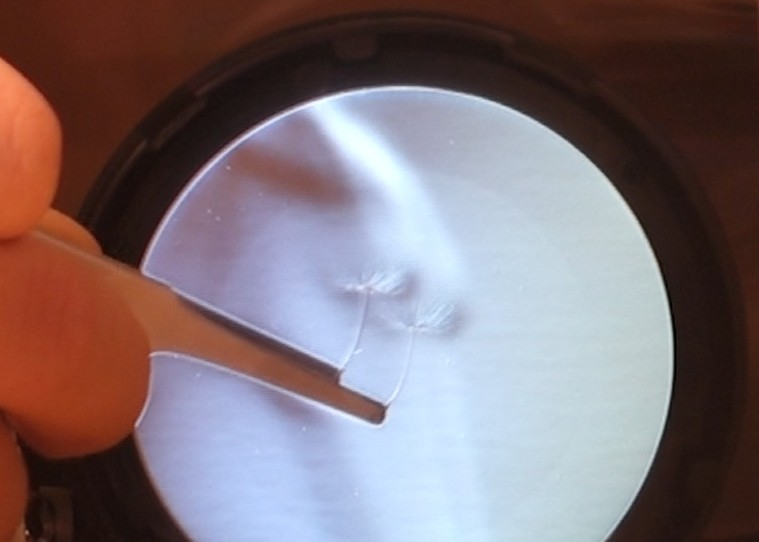
\includegraphics[width=0.6\textwidth]{schliere}
    \caption{Beste Aufnahme mit meinem System, [\textit{Eigene Darstellung}]}
    \label{fig:sl}
\end{figure}

\begin{figure}[h]
    \centering
    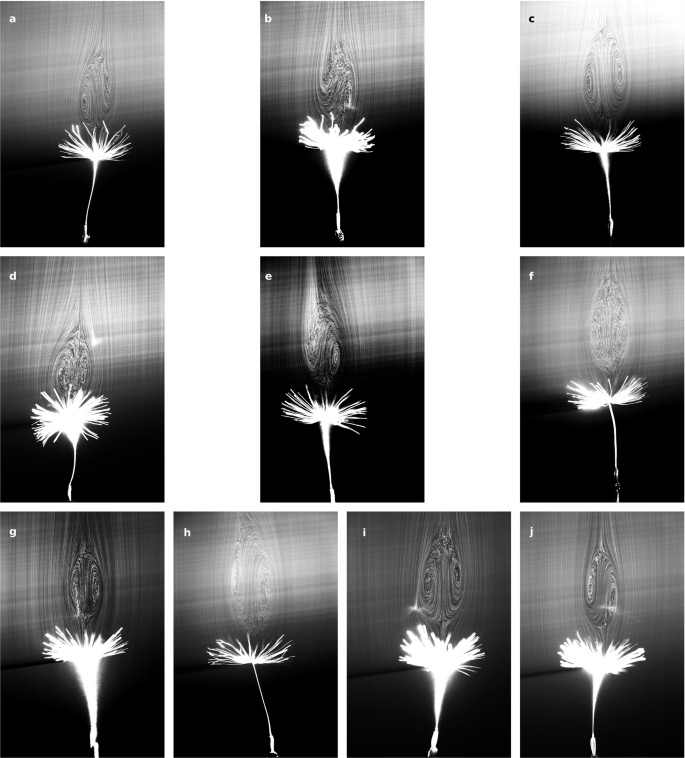
\includegraphics[width=0.5\textwidth]{41586_2018_604_Fig5_ESM}
    \caption{Aufnahmen von profis \footfullcite[, Extended Data Fig. 1]{sl_pro}}
    \label{fig:sl_pro}
\end{figure}
\newpage


    \section{Fazit und Ausblick}\label{sec:anwendung}

    Es ist bedauerlich, dass die im Experiment genutzten Instrumente keine sinnvollen Daten sammeln konnten.
    Dennoch gibt es viele weitere Dokumente die dieselben oder gar mehr Experimente in einer optimalereren Umgebung mit besseren Gerätschaften machen.\\
    Von der Technik aus gesehen hat der Flug der Pusteblume viele chancen.
    Mit der Miniaturisierung von Elektronik könnte man Flugroboter bauen, die nur durch Solarenergie schweben.
    Und es wird auch gesagt, dass die eigenschaften des Pappus einer Platte mit löchern ähneln\footfullcite{tesi},
    was relativ einfach herzustellen ist.\\
    Aber wenn man so tief in Technisches einsteigen will, sollte man auch bereit sein, sodass es nicht wie die experimente hier endet.


    \newpage%%%%%%%%%%%%%%%%%%%%%%%%%%%%%%%%%%%%%%%%%%%%%%%%%%%%%%%%%%%%%%%%%%%%%%%%%%%%%%%%%%%%%%%%%%%%%%%%%%%%%%%%%%%%
    \printbibliography

    \newpage%%%%%%%%%%%%%%%%%%%%%%%%%%%%%%%%%%%%%%%%%%%%%%%%%%%%%%%%%%%%%%%%%%%%%%%%%%%%%%%%%%%%%%%%%%%%%%%%%%%%%%%%%%%%
    \noindent\Large
    Ich erkläre hiermit, dass ich die Seminararbeit ohne fremde Hilfe angefertigt und nur die im Literaturverzeichnis angeführten Quellen und Hilfsmittel benutzt habe.

    \large
    \vspace{\fill}
    \noindent
    \begin{minipage}[b]{0.42\textwidth}
        \centering
        \textit{Nürnberg, \today}
        \vspace{4mm}
        \hrule
        \vspace{2mm}\par\noindent
        Ort, Datum
    \end{minipage}
    \hfill
    \begin{minipage}[b]{0.42\textwidth}
        \centering
        \hrule
        \vspace{2mm}\par\noindent
        Unterschrift des Verfassers
    \end{minipage}
\end{document}
